% Horizon penetrating coordinates (vs. Schwarzschild coordinates)
% for a black hole spacetime, with excision
% Author: Jonah Miller
\documentclass[tikz,border=10pt]{standalone}
%%%<
\usepackage{verbatim}
%%%>
\begin{comment}
:Title: Excised, Horizon-Penetrating Coordinates for Black Hole Spacetime
:Tags: Physics;Decorations;Paths
:Author: Jonah Miller
:Slug: spacetime

This is a "Penrose" or "conformal" diagram for a black hole
spacetime in general relativity. In these diagrams, the top of the
plot is the future and the bottom of the plot is the past. Light
travels along lines at 45 degrees off of the y-axis.

In general relativity, spacetime can be cut up into slices in many
different ways. This plot shows two popular ones: Schwarzschild
coordinates and Kerr-Schild coordinates. It also shows a popular way
of avoiding the black hole singularity via "excision" where the
spacetime is terminated at some finite radius behind the event
horizon. 
\end{comment}
\usetikzlibrary{decorations.pathmorphing}

\tikzset{zigzag/.style={decorate, decoration=zigzag}}
\def \L {2.}

% fix for bug in color.sty
% see: http://tex.stackexchange.com/questions/274524/definecolorset-of-xcolor-problem-with-color-values-starting-with-f
\makeatletter
\def\@hex@@Hex#1%
 {\if a#1A\else \if b#1B\else \if c#1C\else \if d#1D\else
  \if e#1E\else \if f#1F\else #1\fi\fi\fi\fi\fi\fi \@hex@Hex}
\makeatother

% Define a prettier green
\definecolor{darkgreen}{HTML}{006622}

\begin{document}
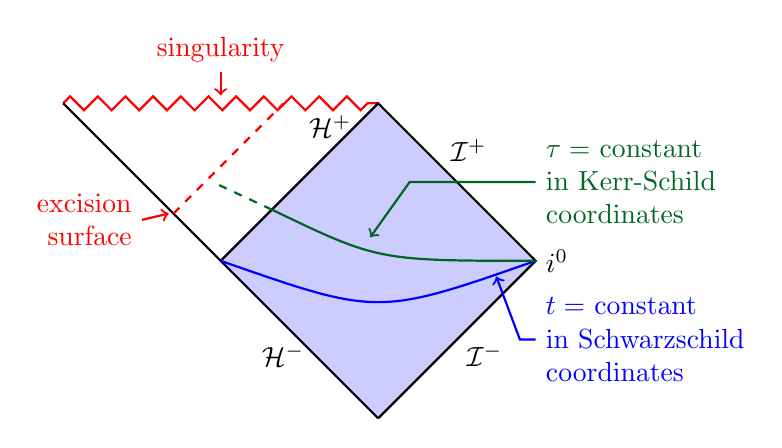
\begin{tikzpicture}

  % causal diamond
  \draw[thick,red,zigzag] (-\L,\L) coordinate(stl) -- (\L,\L) coordinate (str);
  \draw[thick,black] (\L,-\L) coordinate (sbr)
    -- (0,0) coordinate (bif) -- (stl);
  \draw[thick,black,fill=blue, fill opacity=0.2,text opacity=1] 
    (bif) -- (str) -- (2*\L,0) node[right] (io) {$i^0$} -- (sbr);

  % null labels
  \draw[black] (1.4*\L,0.7*\L) node[right]  (scrip) {$\mathcal{I}^+$}
               (1.5*\L,-0.6*\L) node[right] (scrip) {$\mathcal{I}^-$}
               (0.2*\L,-0.6*\L) node[right] (scrip) {$\mathcal{H}^-$}
               (0.5*\L,0.85*\L) node[right] (scrip) {$\mathcal{H}^+$};

  % singularity label
  \draw[thick,red,<-] (0,1.05*\L) 
    -- (0,1.2*\L) node[above] {\color{red} singularity};
  % Scwharzschild surface
  \draw[thick,blue] (bif) .. controls (1.*\L,-0.35*\L) .. (2*\L,0);
  \draw[thick,blue,<-] (1.75*\L,-0.1*\L)  -- (1.9*\L,-0.5*\L)
    -- (2*\L,-0.5*\L) node[right,align=left]
    {$t=$ constant\\in Schwarzschild\\coordinates};
  % excision surface
  \draw[thick,dashed,red] (-0.3*\L,0.3*\L) -- (0.4*\L,\L);
  \draw[thick,red,<-] (-0.33*\L,0.3*\L) 
    -- (-0.5*\L,0.26*\L) node[left,align=right] {excision\\surface};
  % Kerr-Schild surface
  \draw[darkgreen,thick] (0.325*\L,0.325*\L) .. controls (\L,0) .. (2*\L,0);
  \draw[darkgreen,dashed,thick] (0.325*\L,0.325*\L) -- (-0.051*\L,0.5*\L);
  % Kerr-Schild label
  \draw[darkgreen,thick,<-] (0.95*\L,0.15*\L) -- (1.2*\L,0.5*\L)
    -- (2*\L,0.5*\L) node[right,align=left]
    {$\tau=$ constant\\in Kerr-Schild\\coordinates};
\end{tikzpicture}
\end{document}
